
\chapter{準備}
\label{chap:preliminary}
本章では,後の章に向けての準備をする.はじめに,グラフ理論の基本事項を説明する.
・・・などを含む.次に,Cerfらが提唱した一般化ムーアグラフの定義を与え,
いくつかの性質を証明する.これらの性質は,一般化ムーアグラフを探索する方法に
用いるもので,極めて重要である.

\section{グラフ理論の基本事項}
\label{sect:basic-graph-theory}
グラフ理論の基本事項を,\cite{Diestel2000}に則り説明する.
グラフ理論の基礎を理解している読者は\ref{sect:generalized-moore-graph}節まで
読み飛ばしても差し支えない.

\section{一般化ムーアグラフ}
\label{sect:generalized-moore-graph}
本節では一般化ムーアグラフを定義する.
さらに,これが満たすいくつかの性質を示す.

\begin{definition}[Cerf et.al., 1973\,\cite{cerf1973computer}]
  \label{def:generalized-moore-graph}
  次の性質が成り立つ頂点数$n$,次数$k$の正則グラフを
  \textbf{一般化ムーアグラフ}(\textbf{Generalized Moore graph})とよぶ.

  すべての頂点$v$について,$v$から$i$離れた頂点の数
  $c_i = \lvert\{ w\,|\,d(v,w) = i , w\in V \}\rvert$について,
  \[ \begin{cases}
    c_i = k(k-1)^{i-1} & 1\leq i\leq Q \\
    c_{Q+1} = R & \\
    c_i = 0 & Q+2\leq i \leq n-1
  \end{cases} \]
  であること.ただし,
  \begin{align*}
    Q(n,k) &= \max\{q | n-1-\sum_{i=1}^{q}k(k-1)^{i-1} \geq 0\} \\
    R(n,k) &= n - 1 - \sum_{i=1}^{Q(n,k)}k(k-1)^{i-1}
  \end{align*}
  とする.
\end{definition}
\begin{example}
  頂点数12,次数3の一般化ムーアグラフを考える.そのようなグラフを
  \begin{figure}
    \centering
    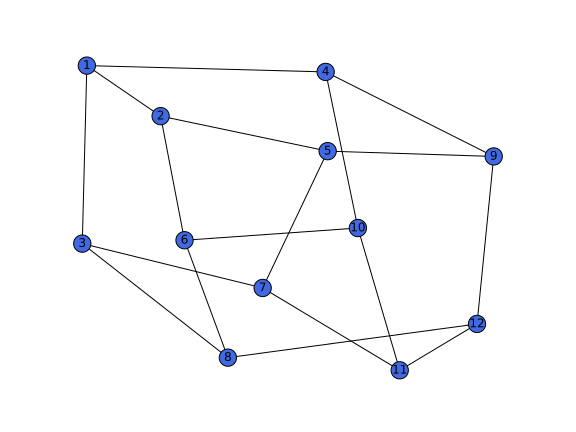
\includegraphics[width=.6\textwidth]{moore-graph-example.pdf}
    \caption{頂点数12,次数3の一般化ムーアグラフの例}
    \label{fig:moore-graph-example}
  \end{figure}
  図\ref{fig:moore-graph-example}に示したグラフを考える.
  $Q(12,3)$と$R(12,3)$はそれぞれ,
  \begin{align*}
    Q(12,3) &= \max\{q | 12-1-\sum_{i=1}^{q}3\cdot2^{i-1} \geq 0\} = 2 \\
    R(12,3) &= 12 - 1 - \sum_{i=1}^{Q(12,3)}3\cdot2^{i-1} = 2
  \end{align*}
  である.このグラフの頂点$1$に着目する.頂点$1$からの距離によって,
  残りの頂点を分類する.
  \begin{enumerate}
  \item 頂点$1$からの距離が$1$の頂点は$\{2,3,4\}$
  \item 頂点$1$からの距離が$2$の頂点は$\{5,6,7,8,9,10\}$
  \item 頂点$1$からの距離が$3$の頂点は$\{11,12\}$
  \end{enumerate}
  である.$1$からの距離が$i$の頂点数$c_i$は,
  \begin{align*}
  c_1 &= 3\cdot2^0 = 3 & \\
  c_2 &= 3\cdot2^1 = 6 & \\
  c_3 &= R(12,3) = 2 & \\
  c_i &= 0 & (i>3)
  \end{align*}
  となるので,定義\ref{def:generalized-moore-graph}で示した距離と頂点数の
  関係を満たす.同様に,他のすべての頂点について,上述の距離と頂点数の関係を
  満たすので,このグラフは一般化ムーアグラフである.
\end{example}
以下,$M(n,k)$を,頂点数$n$,次数$k$の一般化ムーアグラフと記し,
$Q(n,k)$と$R(n,k)$の意味を定義\ref{def:generalized-moore-graph}のとおりとする.
頂点数と次数が文脈から明らかな場合は省略してそれぞれ$M,Q,R$と表す.

一般化ムーアグラフの頂点間距離の総和を求め,これが正則グラフの頂点間距離の総和の
下界であることを示す.
\begin{theorem}[Cerf et.al., 1974\,\cite{Cerf1974}]
  \label{theorem:gmg-lower-bound}
  $M(n,k)$の頂点間距離の総和は,
  \[\sum_{(s,t)\in V\times V}d(s,t) =
  n \left[\ \sum^{Q}_{i=1}ik(k-1)^{i-1} + QR\ \right] \]
  で与えられる.これは,正則グラフの頂点間距離の総和の下界である.
\end{theorem}
\begin{proof}
  眠いまた今度
\end{proof}

次の性質は,一般化ムーアグラフに存在しうる閉路の長さを定める.
後に説明する探索方法に用いる極めて重要な性質である.
\begin{theorem}
  \label{theorem:gmg-geometric-property}
  一般化ムーアグラフに長さ$2Q$以下の閉路は存在しない.

\end{theorem}
\begin{proof}
  眠いまた今度
\end{proof}
